\documentclass{article}
\usepackage[a4paper, total={6in, 8in}]{geometry}
\usepackage{amsmath,amssymb, amsfonts}
\usepackage{fancyhdr}
\usepackage{graphicx}
\graphicspath{ {./images/} }
\usepackage{float}
\usepackage{hyperref}

\pagestyle{fancy}
\fancyhf{}
\rhead{claudeon}
\lhead{DSA1101 Summary}
\rfoot{Page \thepage}
\usepackage{amsmath, amssymb, amsfonts, listings}
\usepackage{xcolor}

%New colors defined below
\definecolor{codegreen}{rgb}{0,0.6,0.4}
\definecolor{codegray}{rgb}{0.5,0.5,0.5}
\definecolor{codepurple}{rgb}{0.58,0,0.82}
\definecolor{backcolour}{rgb}{0.95,0.95,0.92}
\definecolor{commentgreen}{rgb}{0.4,0.8,0.6}
%Code listing style named "mystyle"
\lstdefinestyle{mystyle}{
  backgroundcolor=\color{backcolour},   
  commentstyle=\color{red},
  keywordstyle=\color{blue},
  numberstyle=\tiny\color{codegray},
  stringstyle=\color{codegreen},
  basicstyle=\ttfamily,
  breakatwhitespace=false,         
  breaklines=true,                 
  captionpos=b,                    
  keepspaces=true,                 
  numbers=left,                    
  numbersep=5pt,                  
  showspaces=false,                
  showstringspaces=false,
  showtabs=false,                  
  tabsize=2
}

%"mystyle" code listing set
\lstset{style=mystyle}

\title{CS2040 CheatSheet}
\author{Claudeon R Susanto}
\date{}

\begin{document}

%\maketitle
\tableofcontents
\section{Fundamentals}
\subsection{Basic Statistics}
$$\texttt{mean}(x) = \texttt{sum}(x)\texttt{/length}(x) = \frac{1}{N} \sum_{i=1}^{N}x_i$$
\begin{equation*}
    \begin{split}
        \texttt{median}(x) & = \left\{
        \begin{array}{ll}
            X_{(\frac{N+1}{2})} & \text{if $N$ is odd}\\
            \frac{X_{\frac{N}{2}} + X_{(\frac{N}{2} + 1)}}{2} & \text{if $N$ is even}
        \end{array}
        \right.
    \end{split}
\end{equation*}
$$\texttt{var}(x) = \frac{1}{N-1}\sum_{i=1}^{N}(x_i - \overline{x})^2$$
$$\texttt{sd}(x) = \sqrt{\texttt{var}(x)}$$
$$\texttt{range}(x) = \texttt{max}(x) - \texttt{min}(x)$$
$$\texttt{cov}(x,y) = \frac{1}{N-1}\sum_{i=1}^{N}(x_i - \overline{x})(y_i - \overline{y})$$
$$\texttt{cor}(x,y) = \frac{\texttt{cov}(x,y)}{\texttt{sd}(x) \texttt{sd}(y)}$$
*Note that $\texttt{var}$, $\texttt{cov}$, and $\texttt{cor}$ are calculated from sample, not population.
\subsection{Data Manipulation}
\begin{lstlisting}[language = R]
# import a CSV file of the total annual sales
setwd("c:/data")
sales <- read.csv("yearly_sales.csv")

# extract data
sales$gender      # extract gender data
sales[,4]         # extract 4th dataframe column
sales[1:2,]       # extract 1st two rows of dataframe
sales[,c(1,3,4)]) # extract 1st, 3rd and 4th columns of dataframe
# extract total sales and gender columns
sales[,c("sales_total","gender")] 
# extract all records whose gender is female
sales[sales$gender=="F",] 
# extract all records with total sales above 500
sales[sales$sales_total>500,]

# display all the different categories in a variable
levels(sales$gender)
levels(sales[,4])

\end{lstlisting}

\subsection{Data Visualization}
\begin{figure}[H]
    \centering
    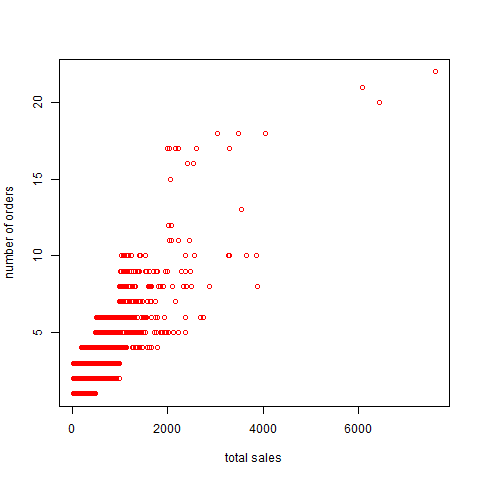
\includegraphics[width=5.5cm]{images/scatter_sales.png}
    \caption{Scatter plot}
\end{figure}
\begin{lstlisting}[language = R]
# simple scatter plot of number of sales versus total sales
png("scatter_sales.png")
plot(x=sales$sales_total, y=sales$num_of_orders, xlab="sales total", ylab="number of orders", col="red", pch=1, main="Title") 
    # lab = label, col = color,
    # pch = point symbols, main = title
dev.off() # shuts down devices
\end{lstlisting}

\begin{figure}[ht]
    \centering
    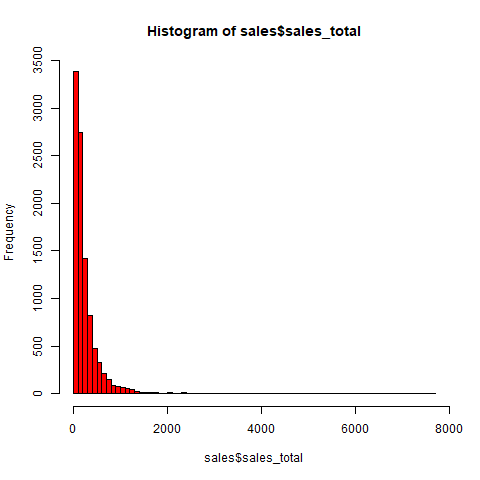
\includegraphics[width=5.5cm]{images/hist2_sales.png}
    \caption{Histogram}
\end{figure}
\begin{lstlisting}[language = R]
# histogram of total sales
png("hist_sales.png")
hist(x=sales$sales_total, breaks=100, col="red")
    # breaks = bins, more breaks more boxes
dev.off()
\end{lstlisting}

\begin{figure}[H]
    \centering
    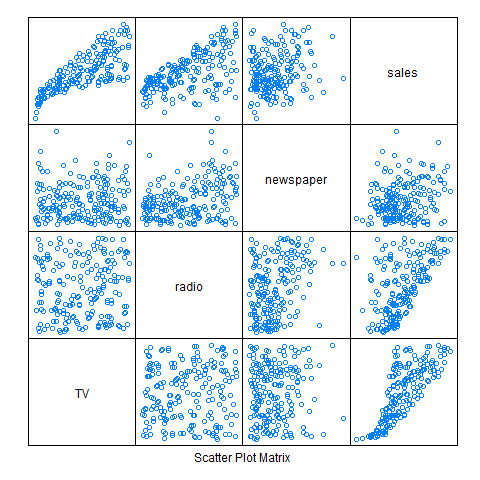
\includegraphics[width=6cm]{images/scatter.png}
    \caption{Pair-wise scatter plots}
\end{figure}
\begin{lstlisting}[language = R]
advert = read.csv("Advertising.csv")
png("scatter.png")
# load package before using the splom function
library(lattice) 
# skip ID line, so just columns 2,3,4,5 in data
splom(~advert[,c(2:5)], groups=NULL, data=advert, axis.line.tck=0, axis.text.alpha=0)
dev.off()
\end{lstlisting}

\subsection{Statistical Learning Methods}
\begin{center}
\begin{tabular}{ c|c } 

 \textbf{Supervised} & \textbf{Unsupervised}\\
 \hline
 Linear regression & $k$-means\\
 \hline
 Decision trees & Association rules\\
 \hline
 $k$-nearest neighbor & Hierarchical clustering\\
 \hline
 Linear discriminant analysis & Deep belief nets\\
 \hline
 Naive Bayes & Self-organizing maps\\
 \hline
\end{tabular}
\end{center}
\begin{itemize}
    \item Supervised learning: making predictions about the outcome $y$ based on a number of predictors
    \item Unsupervised learning: inferring hidden structure based on data without the outcome $y$ ('unlabeled' data)
\end{itemize}


\section{Linear Regression}
\subsection{Simple Linear Regression}
\begin{lstlisting}[language = R]
# basic summary of beta values
lm(sales~TV, data=advert)

# create a summary of t-statistics
linear.reg <- lm(sales~TV, data=advert)
summary(linear.reg)

# more precise values of t-statistics
> summary(linear.reg)$coef

              Estimate  Std. Error  t value    Pr(>|t|)
(Intercept) 7.03259355 0.457842940 15.36028 1.40630e-35
TV          0.04753664 0.002690607 17.66763 1.46739e-42

\end{lstlisting}
\subsubsection{Formulae}
$$\hat{y} = \hat{\beta_0} + \hat{\beta_1} x +\epsilon, \text{ where } \epsilon \thicksim \mathcal{N}(0, \sigma^2 )$$
$$\text{Residual Sum of Squares (RSS)} = \sum_{i=1}^{n}[y_i-(\hat{\beta_0} + \hat{\beta_1}x_i)]^2$$
$$\hat{\beta_1} = \frac{\sum_{i=1}^{n} x_iy_i - \overline{y}\sum_{i=1}^{n} x_i}{\sum_{i=1}^{n} x_i^2 - \overline{x}\sum_{i=1}^{n} x_i}$$
$$\hat{\beta_0} = \overline{y} - \hat{\beta_0}\overline{x}$$
* Std. Error $=$ Standard Error of the Mean (SE).\\
** The $z$-distribution, also called the standard normal distribution, is a special normal distribution where $\mu = 0$ and $\sigma = 1$.\\
*** See \url{https://en.wikipedia.org/wiki/Student\%27s_t-distribution} for the definition of $t$-distribution and \url{https://stattrek.com/probability-distributions/t-distribution.aspx} for more info.

\subsubsection{Hypothesis Testing}
We test the null hypothesis of $H_0: \beta_1 = 0$ versus $H_a: \beta_1 \neq 0$ and compute the $\textit{t-statistic}$ given by:
$$t = \frac{\hat{\beta_1}-0}{\text{SE}(\hat{\beta_1})}$$
where the statistic $t$ has a \textit{t}-distribution with $(n-2)$ degrees of freedom for simple linear regression. Then we can compute the \textit{p}-values directly from the \textit{t}-statistic or use the \texttt{pt()} function in R.
\begin{itemize}
    \item If \textit{p}-value $< \alpha$, then we reject $H_0$ and conclude that there is a linear relationship between $x$ and $y$ at the $\alpha$ significance level.
\end{itemize}


\subsubsection{Confidence Interval}
\begin{lstlisting}[language=R]
> linear.reg <- lm(sales^TV, data=advert)
> new_pt = data.frame(TV=200)
> predict(linear.reg, new_pt, level=0.95, interval="confidence")
       fit      lwr      upr
1 16.53992 16.00567 17.07418

> predict(linear.reg, new_pt, level=0.95, interval="prediction")
       fit      lwr      upr
1 16.53992 10.09162 22.98822

\end{lstlisting}

\subsubsection{Model Diagnostics}
\begin{itemize}
    \item The quality of a linear regression fit can be assessed using the Residual Standard Error (RSE).
$$\text{RSE} = \sqrt{\frac{1}{n-2} \text{RSS}}$$

\item Total Sum of Squares (TSS) measures the total variance in the response $Y$.
$$\text{TSS} = \sum_{i=1}^{n} (y_i - \bar{y})^2$$

\item The $R^2 $ statistic is another measure of the fit of the model. Larger $R^2$ indicates better model fit. Note that $0 \leq R^2 \leq 1$.
$$R^2 = \frac{\text{TSS} - \text{RSS}}{\text{TSS}} = 1- \frac{\text{RSS}}{\text{TSS}}$$
\end{itemize}
\begin{lstlisting}[language = R]
# from summary(linear.reg),
...
Residual standard error: 3.259 on 198 degrees of freedom
Multiple R-squared:  0.6119,    Adjusted R-squared:  0.6099 
F-statistic: 312.1 on 1 and 198 DF,  p-value: < 2.2e-16
\end{lstlisting}

We have assumed that the error term $\epsilon$ is normally distributed with $\mu =0$ and constant variance $\sigma^2$. There are three ways to check:
\begin{enumerate}
\item Plot residuals against fitted values, see if the residuals are observed somewhat \underline{evenly} on both sides of the reference zero line, and the spread of the residuals is \underline{fairly constant} from one fitted value to the next.
\begin{figure}[H]
    \centering
    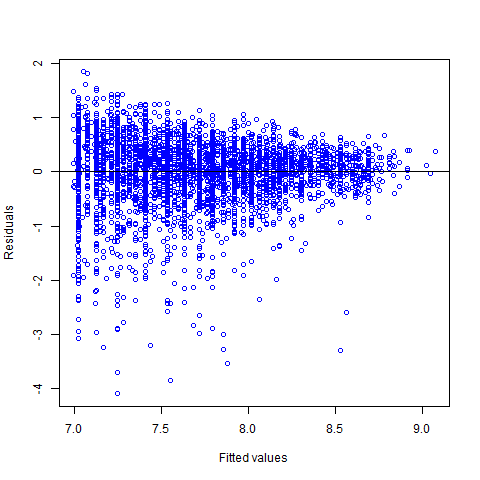
\includegraphics[width=6cm]{images/residuals2.png}
    \caption{Residuals against fitted values}
\end{figure}
\begin{lstlisting}[language=R]
> png("residuals.png")
> plot(x=linear.reg$fitted.values, y=linear.reg$residuals, xlab="Fitted values", ylab="Residuals", col="red")
> abline(0,0) # sketch the line y=ax+b: abline(a,b)
> dev.off()
\end{lstlisting}

\item Histogram of residuals to check the normality assumption for the error terms.
\begin{figure}[H]
    \centering
    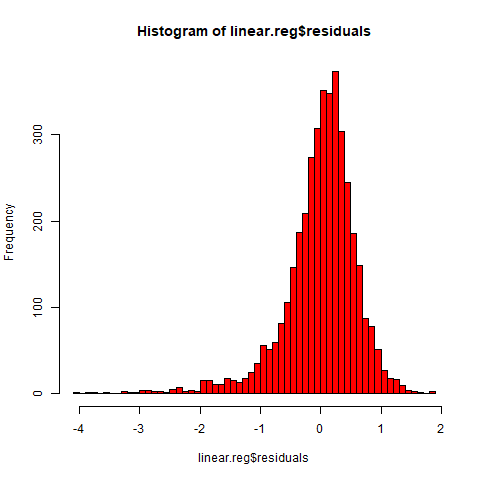
\includegraphics[width=6cm]{images/hist_residuals.png}
    \caption{Histogram of residuals}
\end{figure}
\begin{lstlisting}[language=R]
> png("hist_residuals.png")
> hist(x=linear.reg$residuals, breaks=50, col="red")
> dev.off()
\end{lstlisting}

\item Quantile-Quantile (QQ) plot that compares the observed residuals against the quantiles of the theoretical normal distribution.
\begin{lstlisting}[language=R]
> png("qq_residuals.png")
> qqnorm(linear.reg$residuals, ylab="Residuals", main=" ")
> qqline(linear.reg$residuals)
> dev.off()

\end{lstlisting}

\end{enumerate}

\subsection{Multiple Linear Regression}

\begin{lstlisting}[language= R]
> resale <- read.csv("hdbresale_reg.csv")
> out <- lm(resale_price~town+floor_area_sqm+flat_type, data=resale)

# compute confidence intervals on the parameters
> confint(out, level=0.95)

# provide confidence interval on expected predicted values
> new_pt <- data.frame(town="CENTRAL AREA", flat_type="3 ROOM", floor_area_sqm=70)
> predict(out, new_pt, level=0.95, interval="confidence")
> predict(out, new_pt, level=0.95, interval="prediction")
\end{lstlisting}
In a model with $p$ input variables,
$$y = \beta_0 + \beta_1x(1) + \beta_2x(2) + \dots + \beta_px(p) + \epsilon,$$
\begin{center}
    where $x(j)$ are the input variables, $j = 1,2,\dots, p$
\end{center}

\section{\textit{K}-means Clustering}

\begin{figure}[H]
    \centering
    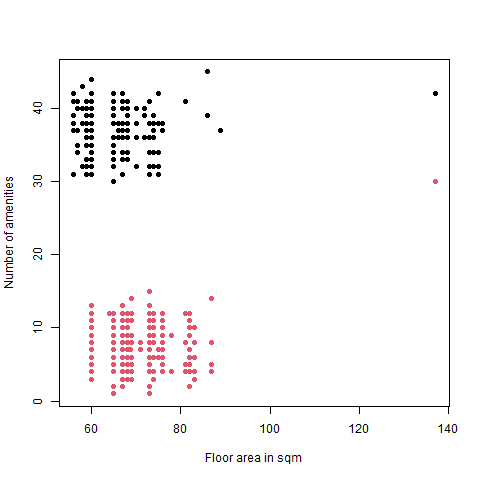
\includegraphics[width=6cm]{images/resale_kmeans.png}
    \caption{$K$-means clustering}
\end{figure}
\begin{lstlisting}[language = R]
resale <- read.csv("hdbresale_cluster.csv")
kout <- kmeans(resale[,c("floor_area_sqm", "amenities")], centers=2)
plot(resale$floor_area_sqm, resale$amenities, 
     col=kout$cluster, 
     xlab="Floor area in sqm", 
     ylab="Number of amenities", pch=19)
\end{lstlisting}
\subsection{Algorithm} 
\begin{enumerate}
    \item Choose the value of $k$ and the $k$ initial guesses for the centroids
    \item Compute the Euclidean distance from each data point to each centroid
    \item Assign the points to their closest centroids
    \item Compute the centroids in each cluster
    \item Repeat steps 2-4 until the algorithm converges to an answer
\end{enumerate}

\subsection{Determining the Number of Clusters}
For a given point $z_i$ at $(x(1)_i, x(2)_i, \dots, x(p)_i)$ and a centroid $D$ at $(x(1)_d, x(2)_d, \dots, x(p)_d)$, the \underline{distance} between $z_i$ and $D$ is 
$$dist(z_i, D) = \sqrt{\sum_{j=1}^{p} (x(j)_i - x(j)_d)^2}$$
The \underline{centroid} for a cluster of $m$ points, $(x(1)_i, x(2)_i, \dots, x(p)_i)$ for $i = 1,2,\dots, m$ is given by 
$$\left( \frac{1}{m} \sum_{i=1}^{m}x(1)_i,  \frac{1}{m} \sum_{i=1}^{m}x(2)_i, \dots, \frac{1}{m} \sum_{i=1}^{m}x(p)_i\right)$$
For $M$ data points $z_1, z_2, \dots, z_M$ with $p$ features the \underline{Within Sum of Squares (WSS)} is calculated via
\begin{equation*}
    \begin{split}
        \text{WSS} & = \sum_{i=1}^{M}dist(z_i,D_i)^2\\
        & = \sum_{i=1}^{M} \sum_{j=1}^{p}(x(j)_i - x(j)_{D_i})^2
    \end{split}
\end{equation*}

\begin{lstlisting}[language=R]
> grade_input = read.csv("grades_kmean_input.csv")
> kout <- kmeans(grade_input[,c("English", "Math", "Science")], centers = 3)
> kout$withinss
[1] 34806.339 22984.131  6692.589
\end{lstlisting}

\begin{figure}[H]
    \centering
    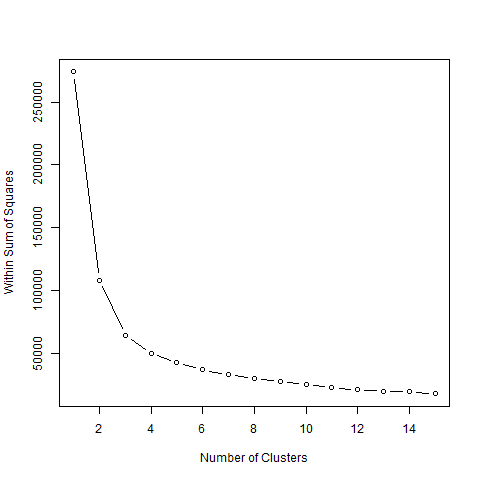
\includegraphics[width=6cm]{images/kmeans.png}
    \caption{WSS against the number of clusters (Elbow curve)}
\end{figure}

\begin{lstlisting}[language=R]
wss <- numeric(15) # creates an array of size 15
for (k in 1:15) {
	km <- kmeans(grade_input[,c("English", "Math", "Science")], centers = k, nstart=25)
	# nstart = do 25 times of K-means clustering
	wss[k] <- sum(km$withinss) # km$tot.withinss
}
plot(1:15, wss, type="b", xlab="Number of Clusters", ylab="Within Sum of Squares")
\end{lstlisting}

\subsection{Feature Selection}
\begin{itemize}
    \item Include only important features, too many attributes can minimize the impact of the most important variables
    \item Identify any highly correlated attributes and only use one or two of them
    \item Choose the appropriate unit of measure for each attribute
    \item Rescale some features so that one feature does not have disproportionate effects on results
\end{itemize}

\section{\textit{K}-nearest Neighbor Classification}
\subsection{Algorithm}
\begin{enumerate}
    \item For two given data points in $p$-dimensional feature space, $z_i$ at $(x(1)_i, x(2)_i, \dots, x(p)_i)$ and $z_j$ at $(x(1)_j, x(2)_j, \dots, x(p)_j)$, the Euclidean distance between $z_i$ and $z_j$ is 
    $$dist(z_i, z_j) = \sum_{l=1}^{p} (x(l)_i - x(l)_j)^2$$
    Find the $k$ nearest neighbors to the data point in the feature space in terms of Euclidean distance
    \item The fitted $\hat{Y}$ with $k$ nearest neighbors for a new data point with feature values $x$ is
$$\hat{Y} = \frac{1}{k} \sum_{z_i \in N_k(x*)}y_i$$
\end{enumerate}
The prediction error of the model can be decomposed into 
$$\text{error} = \text{bias}^2 + \text{variance} + \text{irreducible error}$$
When $k$ increases, the variance decreases but bias increases, this is known as the \underline{bias-variance tradeoff}. There is an inverse relationship between variance and biased

\subsection{Examples}
\begin{itemize}
    \item Example 1: The Stock Market Data
\begin{lstlisting}[language=R]
> market <- read.csv("Smarket.csv")

> train = (market$Year < 2005)
> train.data = market[train,]
> test.data  = market[!train,]

> train.x = train.data[,c("Lag1","Lag2","Lag3","Lag4","Lag5")]
> test.x = test.data[,c("Lag1","Lag2","Lag3","Lag4","Lag5")]
> train.y = train.data[,c("Direction")]
> test.y = test.data[,c("Direction")]

> library(class) # knn() is a function in 'class'
# knn() needs at least 4 args
> knn.pred = knn(train.x, test.x, train.y, k=1)
# create a table for diagnostic of classifier
> confusion.matrix = table(knn.pred, test.y)
> confusion.matrix
        test.y
knn.pred Down Up
    Down   55 66
    Up     56 75
\end{lstlisting}
    \item Example 2: Caravan Insurance Data
\begin{lstlisting}[language=R]
> caravan = read.csv("Caravan.csv")
# exclude ID column, Purchase (Y/N) column
> caravan = caravan[,-1]
> standardized.X = scale(caravan[,-86])
# every column of standardized.X has var=1 and mean=0
\end{lstlisting}
Precision is used as a diagnostic tool here because campaign can be more targeted to potential customers who are more likely to purchase insurance
\item Example 3: Customer Churn\\
Precision as a metric is most useful here because companies can target customers that are more likely to churn by offering various incentives
\begin{lstlisting}[language=R]

\end{lstlisting}
    
\end{itemize}


\subsection{Diagnostics of Classifiers}

\begin{itemize}
    \item The \textit{accuracy} (overall success rate) is a metric defining the rate at which a model has classified the records correctly
    $$\text{Accuracy} = \frac{TP + TN}{TP+TN+FP+FN} \times 100\%$$
    \item The true positive rate (TPR) shows the proportion of positive instances the classifier correctly identified
    $$\text{TPR} = \frac{TP}{TP+FN}$$
    \item The false positive rate (FPR) shows what percentage of negatives the classifier marked as positive. Also called the false alarm rate or the \underline{type I} error rate
    $$\text{FPR} = \frac{FP}{FP+TN}$$
    \item The false negative rate (FNR) shows what percentage of positives the classifier marked as negative. Also called the miss rate or the \underline{type II} error rate
    $$\text{FNR} = \frac{FN}{TP+FN}$$
    \item \textit{Precision} is the percentage of instances marked positive that really are positive
    $$\text{Precision} = \frac{TP}{TP+FP}$$
\end{itemize}

\subsection{\textit{N}-Fold Cross-Validation}
\subsubsection{Algorithm}
\begin{enumerate}
    \item The entire dataset is randomly split into $N$ datasets of approximately equal size.
    \item $N-1$ of these datasets are treated as the \underline{training dataset}, while the remaining one is the \underline{test dataset}. A measure of the model error is obtained.
    \item This process is repeated across the various combinations of $N$ datasets taken $N - 1$ at a time.
    \item The observed $N$ models errors are averaged across the $N$ folds.

\end{enumerate}
\begin{lstlisting}[language=R]
> iris = read.csv("iris.csv", header=FALSE)
> names(iris) = c("X1", "X2", "X3", "X4", "Y")
> library(class)
> X = iris[,c("X1", "X2", "X3", "X4")]
> Y = iris[,c("Y")]

# 150 datapoints are randomly divided into 10 sets
> n_folds=10
> folds_j <- sample(rep(1:n_folds, length.out = 150))
> table(folds_j)
folds_j
 1  2  3  4  5  6  7  8  9 10 
15 15 15 15 15 15 15 15 15 15 
> test_j <- which(folds_j == 1)

> pred <- knn(train=X[-test_j,], test=X[test_j,], cl=Y[-test_j], k=1)
> mean(pred == Y[test_j]) # proportion of datapoints predicted correctly
[1] 0.9333333
> mean(pred != Y[test_j]) # proportion of datapoints predicted incorrectly
[1] 0.06666667
}
\end{lstlisting}
\begin{figure}[H]
    \centering
    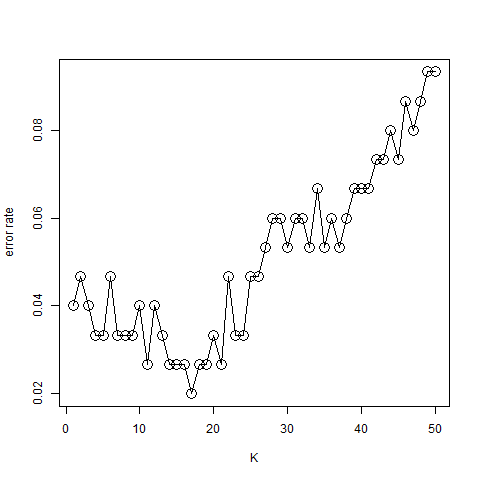
\includegraphics[width=7.5cm]{images/knn_error.png}
    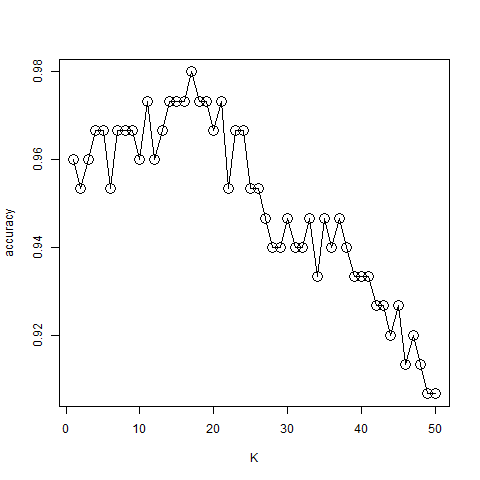
\includegraphics[width=7.5cm]{images/knn_accur.png}
    \caption{KNN: Error rate against different values of K}
\end{figure}
\begin{lstlisting}[language=R]
n_folds=10
folds_j <- sample(rep(1:n_folds, length.out = 150))

error_differentK = numeric(50)
accur_differentK = numeric(50)

for (K in 1:50) {

error = numeric(10)
accur = numeric(10)
for (j in 1:10) {
  test_j <- which(folds_j == j)
  pred <- knn(train=X[-test_j,], test=X[test_j,], cl=Y[-test_j], k=K)
  error[j] = mean(pred != Y[test_j])
  accur[j] = mean(pred == Y[test_j])
}
error_differentK[K] = mean(error)
accur_differentK[K] = mean(accur)

plot(1:50, error_differentK, type="o", ylab="error rate", xlab="K", cex.axis=1, cex=2)
plot(1:50, accur_differentK, type="o", ylab="accuracy", xlab="K", cex.axis=1, cex=2)

\end{lstlisting}

Using the \texttt{caret} library:
\begin{figure}[H]
    \centering
    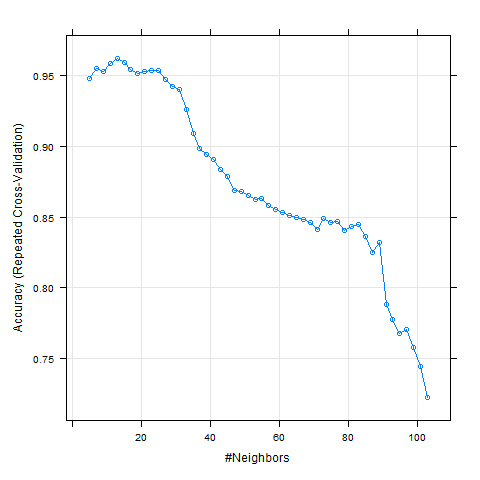
\includegraphics[width=8cm]{images/ncv_caret.png}
    \caption{$N$-fold cross validation using \texttt{caret}}
\end{figure}
\begin{lstlisting}[language=R]
library(caret)

fitControl <- trainControl(## 10-fold cross validation
                           method="repeatedcv",
                           number=10,
                           ## repeated 10 times
                           repeats=10)
set.seed(2)
knnFit1 <- train(Y ~., # predict Y from everything else
                 data=iris, method="knn",
                 trControl=fitControl, #trainControl
                 preProcess=c("center","scale"), # centered & scaled
                 tuneLength=50)
plot(knnFit1)
\end{lstlisting}

\section{Decision Trees}
\subsection{Introduction}
\textbf{‘Branch’} refers to the outcome of a decision and is visualized
as a line connecting two nodes. The branching of a node is referred to as a split.\\
\textbf{'Internal nodes'} are the decision or test points. The topmost internal node is called the root. \\The \textbf{'depth'} of a node is the minimum number of steps required to reach the node from the root. \\\textbf{Leaf nodes} are at the end of the last branches on the tree

\begin{figure}[H]
    \centering
    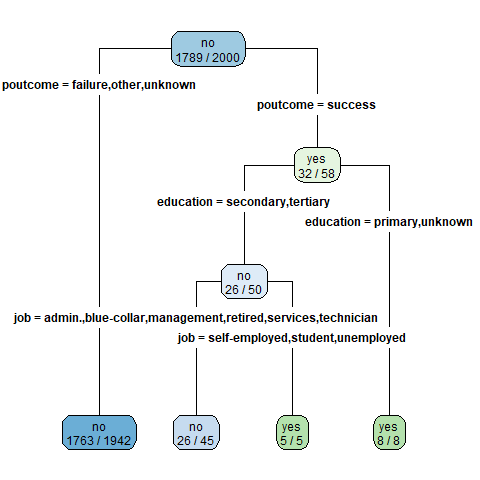
\includegraphics[width=6cm]{images/bankdata.png}
    \caption{Decision Tree}
\end{figure}

\begin{lstlisting}[language=R]
install.packages("rpart")
install.packages("rpart.plot")
# rpart contains functions for modelling decision trees
# rpart.plot enables the plotting of a tree
library("rpart")
library("rpart.plot")

bankdata = read.csv("bank-sample.csv")

fit <- rpart(subscribed~job + marital + education + 
             default + housing + loan + contact + poutcome,
             method="class", data=bankdata,
             control=rpart.control(minsplit=1, maxdepth=4),
               # minsplit =
               # maxdepth = max depth of tree
             parms=list(split="information"))
               # "information" => entropy algo
               # "gini"        => gini algo
rpart.plot(fit, type=4, extra=2, clip.right.labs=FALSE,
           varlen=0, faclen=0)
\end{lstlisting}
\subsection{Algorithm: Entropy}
\begin{itemize}
    \item The \textbf{purity} of a node is defined as its probability of the corresponding class\\
    For example, in the root node, $P(\text{subscribed } = 0) = \frac{1789}{2000}$. Hence the root is $89.45\%$ pure on the subscribed $ = 0$ class and $10.55\%$ pure on the subscribed $ = 1$ class
    \item Given variable $Y$ and the set of possible categorical values it can take, $(y_1, y_2, \dots , y_K)$, the \textbf{entropy} of $Y$ is defined as
    $$D_Y = -\sum_{j=1}^{K}P(Y=y_j)[\log_2P(Y=y_j)]$$
    where $P(Y=y_j)$ denotes the purity or the probability of the class $Y=y_j$ and $\sum_{j=1}^{K}P(Y=y_j)=1$. 
    \begin{itemize}
        \item Heuristically, entropy is a measure of unpredictability. Lower entropy $\Rightarrow$ lower uncertainty and likewise, higher entropy $\Rightarrow$ higher uncertainty
        \item The base entropy is defined as the entropy of the output variable at the root node
    \end{itemize}
    \item Suppose we have a feature variable $X$ and the split values $(x_1,x_2)$. The \textbf{conditional entropy} given feature $X$ and the split points $(x_1, x_2)$ is defined as
    \begin{equation*}
        \begin{split}
            D_{Y|X} &= \sum_{i=1}^{2} P(X=x_i)\cdot D(Y|X=x_i)\\
            &= -\sum_{i=1}^{2}\left\{ P(X=x_i)\sum_{j=1}^{K}P(Y=y_j|X=x_i)\left[\log_2 P(Y=y_j|X=x_i)\right]\right\}
        \end{split}
    \end{equation*}
    \item The reduction in entropy from the base entropy is also known as \textbf{information gain}.
\end{itemize}
Entropy algorithm (from 8.1 slide 38):
\begin{enumerate}
    \item Therefore, the decision tree algorithm proceeds at the root node by calculating the conditional entropy for (i) each feature variable $X$ and (ii) its different split points
    \item Then, the decision variable and its split points are selected based on the largest information gain (or decrease from base entropy)
    \item At internal nodes, the decision tree algorithm proceeds similarly by calculating the conditional entropy for (i) each feature variable $X$ and (ii) its different split points.
    \item However, the sample for calculating the base and conditional entropies is restricted to the one at the node.
    \item The tree is built recursively until a criteria is met, for example:
    \begin{enumerate}
        \item All the leaf nodes in the tree satisfy the minimum purity threshold.
        \item The tree cannot be further split with the preset minimum purity threshold.
        \item Any other stopping criterion is satisfied (such as the maximum depth of the tree).
    \end{enumerate}

\end{enumerate}




\subsection{Algorithm: Gini Index}
\begin{itemize}
    \item Given variable $Y$ and the set of possible categorical values it can take, $(y_1, y_2, \dots, y_K)$, the Gini index of $Y$ is defined as 
    $$G_Y = \sum_{j=1}^{K}P(Y=y_j)[1-P(Y=y_j)]$$
    where $P(Y=y_j)$ denotes the purity or the probability of the class $Y=y_j$ and $\sum_{j=1}^{K}P(Y=y_j)=1$. 
\end{itemize}


\section{Naïve Bayes}
\subsection{Introduction}
\begin{lstlisting}[language=R]
setwd("C:/Users/Claudeon/Downloads")
fruit.dat <- read.csv("fruit.csv")
fruit.dat <- fruit.dat[,-1]
fruit.dat <- data.frame(lapply(fruit.dat, as.factor))
                        # change df to factor
# import library!
library(e1071)

model <- naiveBayes(Fruit~Long+Yellow+Sweet, fruit.dat)

newdata <- data.frame(Long=1, Sweet=1, Yellow=0)
newdata <- data.frame(lapply(newdata, as.factor))

> predict(model, newdata, "raw")
        Banana    Orange    Other
[1,] 0.5284404 0.0587156 0.412844

> predict(model, newdata, "class")
[1] Banana
Levels: Banana Orange Other

# Other Shortcuts!!
> test <- table(fruit.dat[,c("Fruit", "Long")])
> test
        Long
Fruit      0   1
  Banana 300 200
  Orange 280  20
  Other  100 100
> rowSums(test)
Banana Orange  Other 
   500    300    200 
> test/rowSums(test)
        Long
Fruit             0          1
  Banana 0.60000000 0.40000000
  Orange 0.93333333 0.06666667
  Other  0.50000000 0.50000000
\end{lstlisting}
\subsection{Theory}
\begin{itemize}
    \item Assuming conditional independence,
    $$P(AB|C) = P(A|C)P(B|C) \Leftrightarrow P(A|BC) = P(A|C) \leftarrow \text{ definition }$$
    * Event $B$ does not affect $A$ given $C$
    
    \item Assigns a classified label to an object with $m$ feature variables $X = \{X_1, X_2, \dots, X_m\}$ such that the predicted label corresponds to the largest value of $P(Y=y_j|X)$, $j=1,2,\dots,k$ and $Y \in \{y_1, y_2, \dots y_k\}$
    \begin{equation*}
        \begin{split}
            P(Y=y_j|X) &= \frac{P(X_1=x_1,X_2=x_2, \dots, X_m=x_m|Y=y_j)\times P(Y=y_j)}{P(X_1=x_1,X_2=x_2, \dots, X_m=x_m)}\\
            &= \frac{P(Y=y_j)\times \prod_{i=1}^{m}P(X_i=x_i|Y=y_j)}{P(X_1=x_1,X_2=x_2, \dots, X_m=x_m)}\\
            &\propto P(Y=y_j)\times \prod_{i=1}^{m}P(X_i=x_i|Y=y_j)\\
            \Leftrightarrow \log{P(Y=y_j|X)} &= \log{P(Y=y_j)} + \sum_{i=1}^{m} \log{P(X_i=x_i|Y=y_j)}
        \end{split}
    \end{equation*}
    
    \item Ignore denominator term since probability is constant
\end{itemize}

\section{Apriori Algorithm}
\subsection{Introduction}
\begin{lstlisting}[language=R]
library("arules")
library("arulesViz")

data(Groceries) # import Groceries from arules
                # class ==> transaction
# to show/inspect, use Groceries or summary()
> Groceries@itemInfo[1:5,] # shows all the items and their categories
       labels  level2           level1
1 frankfurter sausage meat and sausage
2     sausage sausage meat and sausage
3  liver loaf sausage meat and sausage
4         ham sausage meat and sausage
5        meat sausage meat and sausage
> Groceries@data[10:15,10:15]  # shows items and which 
                               # transactions they're in
                               # in sparse format
6 x 6 sparse Matrix of class "ngCMatrix"
                
[1,] . . . . . .
[2,] . . . | . .
[3,] . . . . . .
[4,] . . . . . .
[5,] . . | . . .
[6,] . | | . . |

# convert sparse format to namelist
# note that column corresponds to transaction no.
#           row corresponds to item no.
> apply(Groceries@data[,101:105], 2, function(r)paste(Groceries@itemInfo[r, "labels"], collapse=", "))
[1] "soda, misc. beverages"                                                                                                 
[2] "sausage, pork, grapes, whole milk, rolls/buns, pastry, soda, specialty bar, bathroom cleaner"                          
[3] "frankfurter, rolls/buns, bottled water"                                                                                
[4] "sausage, whole milk, yogurt, coffee, fruit/vegetable juice, bottled beer, softener, napkins, photo/film, shopping bags"
[5] "soda"   

# Apriori Algorithm
> itemsets <- apriori(Groceries, parameter=list(minlen=1, maxlen=1, support=0.02, target="frequent itemsets"))
    # min/maxlen = min/max length of itemsets
    # target = type of association mined
# inspect items    
> inspect(head(sort(itemsets, by="support"), 5))
    items              support   count
[1] {whole milk}       0.2555160 2513 
[2] {other vegetables} 0.1934926 1903 
[3] {rolls/buns}       0.1839349 1809 
[4] {soda}             0.1743772 1715 
[5] {yogurt}           0.1395018 1372 

# recommended apriori implementation
> itemsets <- apriori(Groceries, parameter=list(minlen=1, support=0.02, target ="frequent itemsets"))
> summary(itemsets)
set of 122 itemsets

most frequent items:
      whole milk other vegetables           yogurt       rolls/buns 
              28               20               11               10 
            soda          (Other) 
              10              108 

element (itemset/transaction) length distribution:sizes
 1  2  3 
59 61  2
...
\end{lstlisting}
\begin{figure}[H]
    \centering
    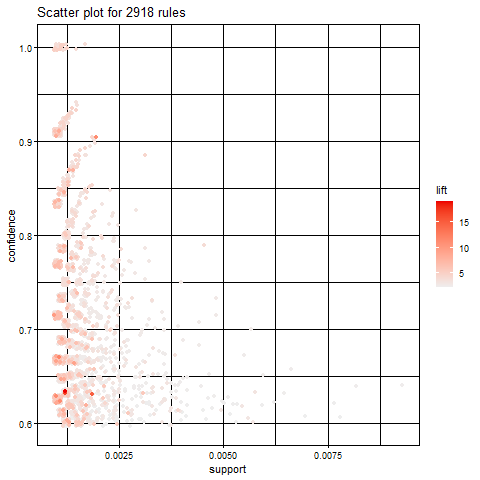
\includegraphics[width=7cm]{images/apriori.png}
    \caption{Association rule scatterplot}
\end{figure}
\begin{lstlisting}[language=R]
> rules <- apriori(Groceries, parameter=list(support =0.001, confidence=0.6, target="rules"))
# lower min support allows more rules to show up
# the highest lift occurs at a low support and a low confidence.
> plot(rules)

# sort association rules by lift
> inspect(head(sort(rules, by="lift"), 3))
    lhs                              rhs              support     confidence
[1] {Instant food products, soda} => {hamburger meat} 0.001220132 0.6315789 
[2] {soda, popcorn}               => {salty snack}    0.001220132 0.6315789 
[3] {ham, processed cheese}       => {white bread}    0.001931876 0.6333333 
    coverage    lift     count
[1] 0.001931876 18.99565 12   
[2] 0.001931876 16.69779 12   
[3] 0.003050330 15.04549 19  
\end{lstlisting}
\subsection{Theory}
\begin{itemize}
    \item Given a $k$-itemset $L=\{i_1,i_2,\dots,i_k\}$, the \textbf{support} of $L$ is the percentage of transactions that contain $L$.
    \item (\textbf{Apriori/Downward Closure Property}) A \textbf{frequent} itemset has items that appear together often enough (when support $>$ minimum support criterion)
    \begin{itemize}
        \item Note that if $X \subseteq Y$ and $Y$ is a frequent itemset then $X$ is also a frequent itemset.
    \end{itemize}
    \item \textbf{Confidence} is defined as the measure of certainty or trustworthiness associated with each discovered rule.
    $$\textit{Confidence}(X\rightarrow Y) = \frac{\textit{Support}(X\wedge Y)}{\textit{Support}(X)}$$
    \item A relationship is thought of as interesting when the algorithm identifies the relationship with a measure of confidence greater than or equal to a predefined threshold.
    \item \textbf{Lift} measures how many times more often X and Y occur together than expected if they are statistically independent of each other ($Lift=1$ means $X$ and $Y$ are statistically independent of each other, the higher the value the more useful the rule is)
    $$Lift(X \rightarrow Y) = \frac{Support(X \wedge Y)}{Support(X)\times Support(Y)}$$
    \item \textbf{Leverage} ($Leverage =0$ means $X$ and $Y$ are statistically independent of each other, larger value indicates stronger relationship)
    $$Leverage(X \rightarrow Y) = Support(X \wedge Y)-Support(X)\times Support(Y)$$
    
\end{itemize}


\section{Additional Resources}
\subsection{Hypothesis Testing}
\begin{itemize}
    \item Steven Walker. 2020. \textit{A Level Maths - hypothesis tests and the art of being non-assertive}. Source: \url{https://www.ocr.org.uk/blog/a-level-maths-hypothesis-tests-and-the-art-of-being-non-assertive/}
    \item Khan Academy. 2018. \textit{Calculating t statistic for slope of regression line}. Source: \url{https://www.youtube.com/watch?v=7MAuojBTF-g}
    \item Khan Academy. 2018. \textit{Using a P-value to make conclusions in a test about slope}. Source: \url{https://www.youtube.com/watch?v=Mpd83AuDTrU}
\end{itemize}


\end{document}